\documentclass[10pt]{article}
\usepackage[polish]{babel}
\usepackage[utf8]{inputenc}
\usepackage[T1]{fontenc}
\usepackage{graphicx}
\usepackage[export]{adjustbox}
\graphicspath{ {./images/} }
\usepackage{amsmath}
\usepackage{amsfonts}
\usepackage{amssymb}
\usepackage[version=4]{mhchem}
\usepackage{stmaryrd}

\title{GIMNAZJUM }

\author{}
\date{}


\begin{document}
\maketitle
\begin{enumerate}
  \item Koło numer 1 ma średnicę 72 mm . Jaką średnicę powinno mieć koło numer 2, aby cały mechanizm działał poprawnie?
  \item Szkoła zakupiła pewną ilość ołówków i postanowiono rozdać je uczniom klas pierwszych. W szkole są trzy klasy pierwsze: la, lb i Ic. Wiadomo, że gdyby ołówki zostały rozdane po równo wszystkim uczniom, każdy otrzymałby po 16 ołówków. Gdyby\\
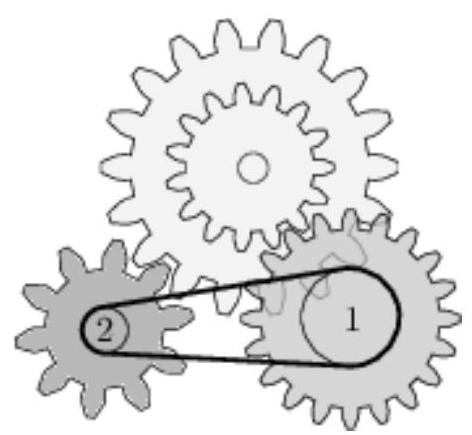
\includegraphics[max width=\textwidth, center]{2024_11_21_380bde68f8bdcfb12cb9g-1}\\
zostały rozdane po równo uczniom klasy la, każdy uczeń tej klasy dostałby po 48 ołówków. Jeśli zostałyby rozdane tylko uczniom klasy lb, każdy z nich otrzymałby po 40 ołówków. Po ile ołówków dostałby każdy uczeń klasy Ic, gdyby postanowiono je rozdać uczniom tylko tej klasy?
  \item Dany jest równoległobok ABCD. Na bokach AB i AD leżą odpowiednio takie punkty X i Y różne od \(A\), że \(A D=D X\) oraz \(A B=B Y\). Udowodnij, że \(C X=C Y\).
\end{enumerate}

\section*{LICEUM}
\begin{enumerate}
  \item Znajdź wszystkie liczby pierwsze \(p\) o tej własności, że liczba \(19 p+1\) jest sześcianem pewnej liczby całkowitej.
  \item Niech \(x\) będzie liczbą rzeczywistą spełniającą równanie \(x^{3}+4 x=8\). Znajdź wartość wyrażenia \(x^{7}+64 x^{2}\).
  \item Dwa kwadraty mają wspólny środek, a wierzchołki mniejszego z nich należą do boków większego. Jeżeli wytniemy z większego kwadratu mniejszy, pozostaną cztery przystające trójkąty, z których każdy ma pole równe 1/12 pola większego kwadratu. Jaką miarę ma najmniejszy z kątów wewnętrznych w każdym z otrzymanych czterech trójkątów?\\
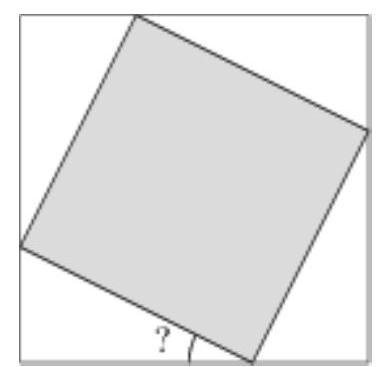
\includegraphics[max width=\textwidth, center]{2024_11_21_380bde68f8bdcfb12cb9g-1(1)}
\end{enumerate}

\end{document}